\chapter{Introduction}\label{cha:intro}
Discrepancies in measurements of the rotations of galaxies indicate the presence of a large amount of matter which interacts through gravity, though not electromagnetically making it invisible to our telescopes. This matter is commonly referred to as dark matter. Since no known or hypothesised particle in the standard model of particle physics can be used as a candidate for dark matter, this has opened the door for new physics. Aside from dark matter there are other phenomena, such as the neutrino mass and the hierarchy problem, that can not be explained today. One of the proposed models to correct these discrepancies is known as Supersymmetry (\abbrSUSY).  

At the Organisation européene pour la recherche nucléaire (\abbrCERN) the interest now lies to discover any evidence of \abbrSUSY. Among other searches one is fixed at looking for so called weakly interacting massive particles (\abbrWIMPS) which may be a candidate for dark matter. It is usually impossible to detect any interaction of dark matter candidates on the subatomic scale, however through looking at proposed interactions, searching for assumed decay channels and inconsistencies in momentum conservation it is hoped that signs will be found. Tough as of \today\ none have been found. 

Both these experiments and current theories now show that higher energies are required at the \abbrLHC to be able to see any signs. This is why the \abbrLHC and all detectors are undergoing a vast upgrading program \textbf{reference!}.
In this thesis, focus will be on the last part of the upgrade due for completion 2023 known as the high luminosity-\abbrLHC phase II upgrade. Also focus lies only with the \abbrATLAS detector.

In this chapter an introduction to both the theoretical and experimental details required to understand the method and results is given. 

\newpage
\section{Research goals}\label{sec:goals}
This research took place at Stockholm University from January 7th until \textbf{when?}
During the research period the following tasks were set up and performed/answered:
\begin{itemize}
\item Implement a C++ programme that loops over the collisions inside the signal and background datasets.	
\item For each collision retrieve the relevant observables (variables used to	 extract the signal over the background) and apply "smearing functions" to emulate the effect of the high luminosity on the observables. 	
\item For both signal and background datasets, compare observables before and after smearing. What observables are the least/most affected?	
\item Implement selection criteria that selects the signal collisions efficiently while reduces significantly the background. In a first step the selection criteria should be taken from existing studies.
\item Selection criteria can be evaluated and compared with each other using a figure of merit Z, that measures the sensitivity of the experiment to the	 dark matter signal. Calculate Z for the given selection criteria before and after smearing.
\item What is the effect of the high luminosity (smearing) on the value of Z?
\item Investigate other selection criteria and observables, to mitigate the effect of high luminosity. Use Z to rank different criteria after smearing.
\item Conclude on the effect of the high luminosity on the sensitivity for dark matter and possible ways to mitigate its effects using alternative observables and selection criteria. 
\end{itemize}
\newpage
\section{Theoretical Background}\label{sec:tb}
The following is a short description of the theory which is required to understand this thesis. 
\subsection{Quantum mechanics and quantum field theory}\label{sec:qm}
\textbf{From my BSc.}

In the beginning of the 20th century, some physical phenomena could not be explained by classical physics, for example the ultra-violet disaster of any classical model of of black-body radiation, and the photoelectric effect.\citep{Bransden:2000}
It was these phenomena that led to the formulation of quantum mechanics (\abbrQM), where energy transfer is quantized and particles can act as both waves and particles at the same time. 

Combining \abbrQM with classical electromagnetism proved harder than expected, colliding a photon(em-field) and an electron (particle/wave) is quite tricky. (Refer to scattering) One idea that came from this was to explain them both in the same framework, field theory.
Also, trying to incorporate special relativity into \abbrQM suggested a field description. (Metric description and bending of gravitational fields).
The culmination of both of these problems is Quantum electrodynamics (\abbrQED)which with incredible precision explains electromagnetic phenomena including effects from special relativity.\citep{Zee:2003}


Something something Lagrangian of these processes something something can be simply viewed through Feynman diagrams.
Explain four-vectors quickly.
Somehow end up with Feynman diagrams.

Also mention special rel + qm expects and now proven antimatter.

Speak about: Why \abbrQM, Lagrangian refer to classical mechanics, end with hand of to particle physics. need to explain observables.
Theoretical Particle physics comes from Feynman diagrams!

Dont forget to explain cross-sections from qft.

Find more information in \citep{Goldstein:2001,Bransden:2000, Zee:2003}.
\subsection{Effective field theory}
In general:
Feynman diagram with a big circle.

From article:


Which one do we use? What parameters have we joined?


How does this pertain to the rest?
info in \citep{82.116010}
\subsection{Nuclear, particle and subatomic particle physics}
Can be seen as the experimental counterpart to quantum mechanics.
Many could argue that these branches started after Ernest Rutherford famous gold foil experiment (reference), where he discovered that matter is composed of matter with a nucleus, a lot of empty space and electrons. This and more sparked the curiosity to see what the nucleus was made of and so on... 

The discovery of the quark diving of bosons/fermions different generations. Fundamental particles. Basically all of 20th century physics. 

Something so that a description of particles are in here, end with standard model.
Content should be enough for the rest of the thesis regarding collisions etc.
Luminosity!

Explain hadrons...

\subsection{The standard model of particle physics} 
How and why is there a standard model? give the Lagrangian and refer to all the different interactions that are included. Which then combines \abbrQM with subatomic particle physics.
 
Mention Antimatter!
Is it proved? What problems exist? 

\subsection{Beyond the standard model: Supersymmetry}
In the early 1970:s similar as \abbrQED expansion with antimatter due to (integral which one diverged?). Similarly to this, an expansion with a similar symmetry having bosons instead of fermions and the reverse. These symmetrical particles are known as supersymmetrical partners. The \abbrSUSY partner of a boson is denoted as sfermion (squarks and sleptons) whereas the \abbrSUSY partner of a fermion is denoted as bosinos (gauginos)

Different problems, hierarchy, etc

Bring up different expansions. Here we will talk about supersymmetry (\abbrSUSY) end with neutrilino/\abbrWIMPS. 
Minimal Supersymmetric Standard Model

Supersymmetry: Every boson has a supersymmetrical fermion, and the reverse.

Some from, else from licentiates \citep{Martin:1998}

\subsection{Dark matter}\label{sec:dark}
A very quick introduction was given in the beginning of this chapter. Dark matter is the name given to the solution to the discrepancies of galactic rotations. 

After this the big question arises, what could this dark matter consist of? 

Weakly interacting massive particles (\abbrWIMPS) are a candidate to explain Dark matter, it is this candidate which is considered in this thesis.
In addition the condition that the WIMPS are Dirac fermions (fermions which are not their own antiparticle) is implied.

In \tableref{tab:operators} the operators which are integrated out via the effective field theory and are of interest in this thesis are given.
\renewcommand{\arraystretch}{1.5} %Change height of tabel
\begin{table}[H]
\begin{center}
    \begin{tabular}{ | l | l | l | l |}
    \hline
    Name & Initial state & Type & Operator \\ \hline
  	D1 & qq & scalar & $\frac{m_q}{M^3_*} \bar{\chi} \chi \bar{q} q$ \\ \hline
  	D5 & qq & vector & $\frac{1}{M^2_*} \bar{\chi} \gamma^\mu \chi \bar{q} \gamma_\mu q$ \\ \hline
  	D8 & qq & axial-vector & $\frac{1}{M^2_*}\bar{\chi}\gamma^\mu \gamma^5 \chi \bar{q} \gamma_\mu \gamma^5 q $ \\ \hline
  	D9 & qq & tensor & $\frac{1}{M^2_*} \bar{\chi}\sigma^{\mu \nu} \chi \bar{q} \sigma_{\mu \nu} q  $\\ \hline
  	D11 & gg & scalar & $\frac{1}{4M^3_*}\bar{\chi}\chi \alpha_s (G^a_{\mu \nu})^2 $\\ \hline
  	\end{tabular}

  	\caption{From \citep{CERN-PH-EP-2012-210}}
  	\label{tab:operators}
  	  	\end{center}
    \end{table}
\renewcommand{\arraystretch}{1.0}  %Back to default
Where D denotes that the \abbrWIMPS are assumed to be Dirac fermions.

Alot here taken from \citep{82.116010}

\subsection{Search for \abbrWIMPS}
Since the search for \abbrWIMPS at the \abbrLHC is based on looking at $E_T^{Miss}$ it will be canonical though the experiment can no establish if a \abbrWIMP is stable on a cosmological time scale and thus if it is a Dark matter candidate \citep{CERN-PH-EP-2012-210}

Include SUSY-feynman?

What is it? Why at \abbrCERN/\abbrATLAS? Candidates?
Dark matter is something which does not interact electromagnetically however it does have a gravitational effect on nearby bodies.
Cold dark matter?
Non-barionic dark matter. Why not barionic?
\abbrWIMPS, wimps as candidates.
How is this detectable at \abbrATLAS? Finish with this. Refer next chapter and that neutralinos are a candidate.

\newpage
\section{Experimental overview}\label{sec:experiment}
What was used in this research and what needs to be explained? Upgrade, pileup etc.
Somewhere here explain how the radial coordinate system is defined.
\subsection{\abbrLHC}
The Large hadron collider (\abbrLHC) is the a particle accelerator located at \abbrCERN near Geneva in Switzerland, see \figureref{fig:lhc}. The accelerator was build to explore physics beyond the standard model and to make more accurate measurements measurements of standard model physics. Before it was shut down for an upgrade in 2012 it was able to accelerate two proton beams to such a velocity that they had an energy of 4 TeV which gives a center of mass energy, $\sqrt{s}=8$ TeV. Apart from the energy, the ability for an accelerator to produce interactions can be calculated through the instantaneous luminosity of the \abbrLHC was $10^{34}$ cm$^{-2}$s$^{-1}$ or $10$nb$^{-1}$s$^{-1}$ where 1 barn(b)$=10^{-24}$ cm$^2$. All values taken from \citep{lumires}.
\begin{figure}[H]
\begin{center}
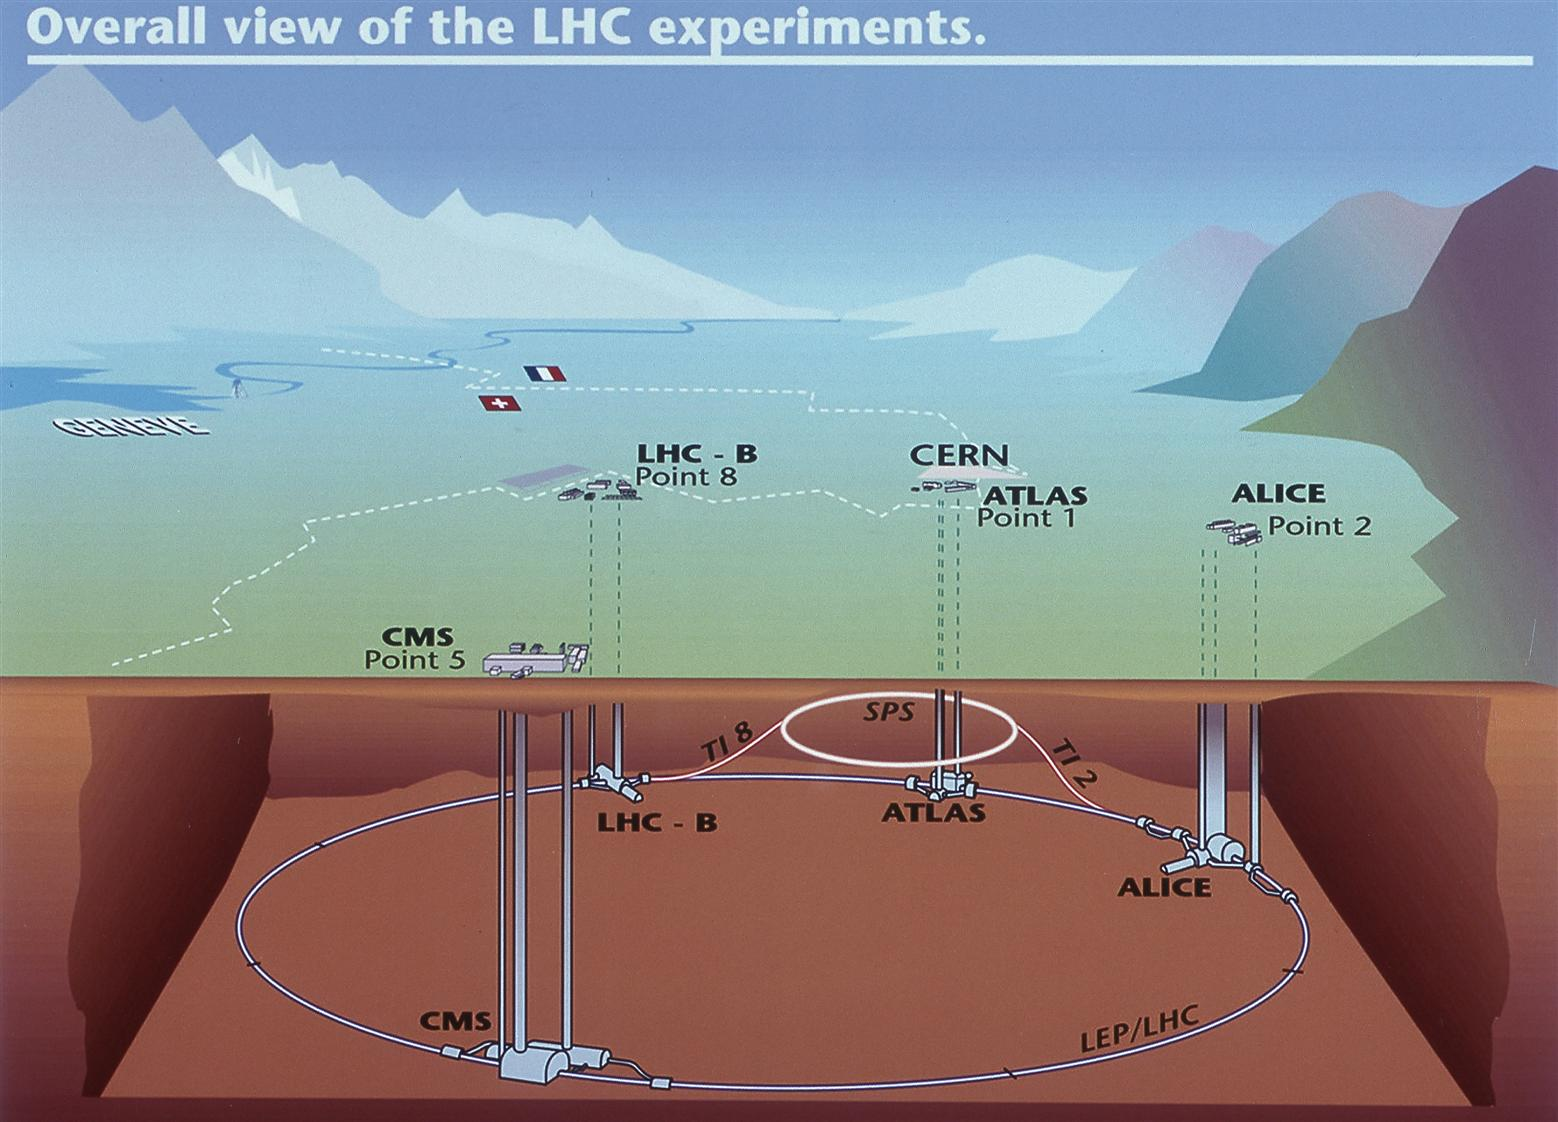
\includegraphics[scale=0.4]{lhc.jpeg}
\caption{Figure showing the \abbrLHC and the different detectors\citep{lhcimage}}
\label{fig:lhc}
\end{center}
\end{figure}
The instantaneous luminosity can be defined in different ways depending on how the collision takes place. For two collinear intersecting particle beams it is defined as:
\textbf{Bunches!}
\begin{equation}
\mathscr{L} = \frac{fkN_1 N_2}{4\pi \sigma_x \sigma_y}
\end{equation}
where $N_i$ are the number of particles in each of the bunches, f is the frequency at which the bunches collide , k the number of colliding bunches in each beam, and $\sigma_x$ ($\sigma_y$) is the horizontal (vertical) beam size at the interaction point. Since the luminosity increases quadratically with more particles in each bunch this would be a good strategy. However aside from the difficulties to create and maintain a beam with more particles, a large $N_i$ increases the probability for multiple collisions per bunch crossing, referred to as pile-up. Pile up will be a key aspect which is described more in \subsectionref{sec:experiment:subsec:pileup}. 

The expected number of events can be calculated by using the instantaneous luminosity through the following:
\begin{equation}
N=\sigma \int \mathscr{L} dt := \sigma \Lagr
\end{equation}
where $\sigma$ is the cross section which is often measured in barn.
The cross section is defined as:
\begin{equation}
\sigma = \oint d\Omega \frac{d\sigma}{d\Omega}
\end{equation}
The cross section is therefore a measure of the effective surface area seen by the impinging particles, and as such is expressed in units of area. The cross section is proportional to the probability that an interaction will occur. It also provides a measure of the strength of the interaction between the scattered particle and the scattering center.
Further details can be found in reference~\citep{Herr:2006}

\subsection{\abbrATLAS}
As seen in \figureref{fig:lhc}, there are several detectors at \abbrCERN. One of these is a large torodial \abbrLHC apparatus (\abbrATLAS) which is a general purpose detector. Its goal is to observe several different production and decay channels. The detector is composed of three concentric subdetectors, the Inner detector, the Calorimeters and the Muon spectrometer.


Most and more in \citep{1129811}
\subsection{Coordinate system}
The coordinate system of ATLAS, seen in \figureref{fig:coordinatesystem} is a right-handed coordinate system with the x-axis pointing towards the centre of the LHC tunnel, and the z-axis along the tunnel/beam (counter clockwise) seen from above. The y-axis points upward.
The origin is define as the interaction point.
A cylindrical coordinate system is also used for the transversal plane. (R,$\phi$,Z).
For simplicity the pseudorapidity of particles from the primary vertex is defined as:
\begin{equation}
\eta = - \ln( \tan\frac{\theta}{2})
\end{equation}
where $\theta$ is the polar angle (xz-plane) of the particle direction measured from the positive z-axis. 
$\eta$ is through this definition invariant under boosts in the z-direction.

It is quite common to calculate the distance between particles and jets in the $(\eta,\phi$) plane, $d=\sqrt{\Delta \eta + \Delta \phi}$  

\begin{figure}[ht]
\begin{center}
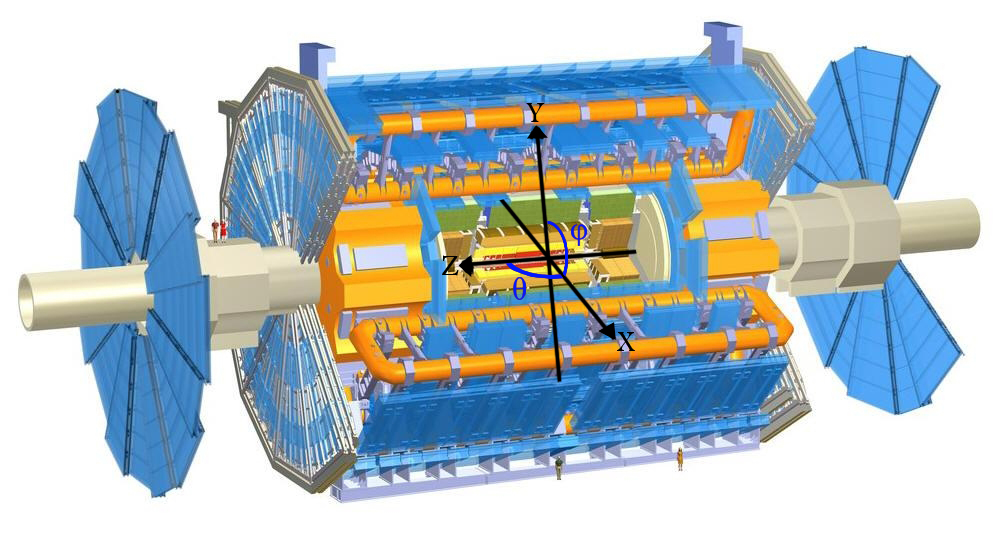
\includegraphics[scale=0.25]{particle_collider.jpg}
\caption{Figure showing the \abbrATLAS detector and the definition of the coordinate system. Image altered from\citep{coordimage}}
\label{fig:coordinatesystem}
\end{center}
\end{figure}

\subsection{Calorimeter}
\subsection{Truth and reconstructed data}
Give a general description.

In this thesis, truth = Montecarlo. 
Reconstructed data = that which is seen in the detectors, which is the smeared data.
\subsection{Pile-up}\label{sec:experiment:subsec:pileup}
\subsection{Jet and missing energy}
What is a jet? why are we only looking at transverse missing energy? 

\subsection{Phase II high luminosity upgrade}
Talk about the upgrade schedule.
I am looking at the upgrade which will be done at \abbrCERN and will be completed around 2022-2023 and is denoted High Luminosity-\abbrLHC Phase 2 upgrade. When this is running the following is expected:
\begin{table}[H]
\begin{center}
    \begin{tabular}{ | l | l | l |}
    \hline
    Entity & Expected & Last run (2012) \\ \hline
  	Luminosity & 1000-3000 fb$^{-1}$ & 20.8 fb$^{-1}$ \\ \hline
  	Pile-up & $\obs{\mu}=200$ & $\obs{\mu}=20.7$ \\ \hline
  	Center of mass energy & $\sqrt{s}=14$ TeV &  $\sqrt{s}=8$ TeV \\ \hline
  	\end{tabular}
  	
  	\caption{Expected running values for the Phase II HL-upgraded \abbrLHC with older values for comparison. REFERENCE?}
  	\label{tab:expectvalues}
  	\end{center}
    \end{table}
Taken from "a short explanation of different terminology by me" Find a cern source.
Assumed effects, timespan when will it be done?
